\documentclass{sig-alternate-05-2015}


\usepackage{times}
\usepackage{graphicx}
\usepackage{latexsym}
\usepackage{xspace}
\usepackage{hyperref}
\usepackage{amssymb}
\usepackage{algorithm}
\usepackage[noend]{algpseudocode}
\usepackage[numbers]{natbib}
\usepackage{notoccite}
\usepackage{framed}
\usepackage{amsmath}
\usepackage{tabularx}

\usepackage[dvipsnames]{xcolor}
\newcommand{\sergey}[1]{\textcolor{magenta}{{\sc Sergey:} #1}\xspace}
\newcommand{\samuel}[1]{\textcolor{green}{{\sc Samuel:} #1}\xspace}
\newcommand{\tias}[1]{\textcolor{blue}{{\sc Tias:} #1}\xspace}
\newcommand{\luc}[1]{\textcolor{red}{{\sc Luc:} #1}\xspace}

\newcommand{\constraints}{\ensuremath{\mathcal{T}}\xspace}
\newcommand{\format}[1]{\textit{#1}\xspace}
\newcommand{\generategroups}{\format{generateGroups}}
\newcommand{\extractgroups}{\format{extractGroups}}
\newcommand{\extracttables}{\format{extractTables}}
\newcommand{\learnconstraints}{\format{learnConstraints}}
\newcommand{\findassignment}{\format{findConstraints}}
\newcommand{\postprocess}{\format{pruneRedundant}}
\newcommand{\constrainttorder}{\format{templateOrder}}
\newcommand{\template}{\format{constraint template}}
\newcommand{\sname}{\format{TaCLe}}


\newcommand{\CName}{Syntax\xspace}
\newcommand{\CSignature}{Signature\xspace}
\newcommand{\CFunction}{Definition\xspace}
\newcommand{\dependencies}{\ensuremath{\mathcal{D}}\xspace}
\newcommand{\groups}{\ensuremath{\mathcal{G}}\xspace}

\newcommand{\range}[3]{\ensuremath{#1[#2,#3]}}
\newcommand{\rangeto}[2]{#1{:}#2}
\newcommand{\rangeall}{:}

\newcommand{\eccalc}[2]{\ensuremath{#1 = #2}}
\newcommand{\ecrank}[2]{\eccalc{#1}{\mathit{RANK}(#2)}}
\newcommand{\ecfkey}[2]{\ensuremath{\mathit{FOREIGNKEY}(#1,#2)}}
\newcommand{\ecalldiff}[1]{\ensuremath{\mathit{ALLDIFFERENT}(#1)}}
\newcommand{\eclookupf}[4]{\ensuremath{\mathit{LOOKUP}_{\mathit{#4}}(#1, #2, #3)}}
\newcommand{\eclookup}[4]{\eccalc{#1}{\eclookupf{#2}{#3}{#4}{}}}
\newcommand{\eclookupprod}[5]{\eccalc{#1}{#2 \times \eclookupf{#3}{#4}{#5}{}}}
\newcommand{\eclookupfuzzy}[4]{\eccalc{#1}{\eclookupf{#2}{#3}{#4}{fuzzy}}}
\newcommand{\ecperm}[1]{\ensuremath{\mathit{PERMUTATION}(#1)}}
\newcommand{\ecseries}[1]{\ensuremath{\mathit{SERIES}(#1)}}
\newcommand{\ecprod}[3]{\eccalc{#1}{#2 \times #3}}
\newcommand{\ecdiff}[3]{\eccalc{#1}{#2 - #3}}
\newcommand{\ectotal}[3]{\eccalc{#1}{\mathit{PREV}(#1) + #2 - #3}}
\newcommand{\ecproj}[2]{\eccalc{#1}{\mathit{PROJECT}(#2)}}
\newcommand{\ecaggc}[3]{\eccalc{#2}{\mathit{#1}(#3, col)}}
\newcommand{\ecaggr}[3]{\eccalc{#2}{\mathit{#1}(#3, row)}}
\newcommand{\ecsumc}[2]{\eccalc{#1}{\mathit{SUM}(#2, col)}}
\newcommand{\ecsumr}[2]{\eccalc{#1}{\mathit{SUM}(#2, row)}}
\newcommand{\ecaggif}[5]{\eccalc{#2}{\mathit{#1IF}(#3, #4, #5)}}
\newcommand{\ecsumif}[4]{\eccalc{#1}{\mathit{SUMIF}(#2, #3, #4)}}
\newcommand{\ecsumprod}[3]{\eccalc{#1}{\mathit{SUMPRODUCT}(#2, #3)}}

\newcommand{\numeric}{\format{numeric}}
\newcommand{\textual}{\format{textual}}
\newcommand{\integer}{\format{integer}}
\newcommand{\discrete}{\format{discrete}}
\newcommand{\plength}{\format{length}}
\newcommand{\ptype}{\format{type}}
\newcommand{\ptable}{\format{table}}
\newcommand{\por}{\format{orientation}}
\newcommand{\prows}{\format{rows}}
\newcommand{\pcols}{\format{columns}}
\newcommand{\nat}{\mathcal{N}}

\newcommand{\sg}{G'}




\renewcommand{\arraystretch}{1.5}

%\usepackage{amsthm} % incompatible with ACM
%\theoremstyle{definition}
%\newtheorem{definition}{Definition}
\newdef{definition}{Definition} % ACM specific


%%\ecaisubmission   % inserts page numbers. Use only for submission of paper.
                  % Do NOT use for camera-ready version of paper.

\begin{document}

\title{Learning constraints in tabular data}
% see http://www.acm.org/binaries/content/assets/publications/article-templates/sig-alternate-sample.tex

%\author{Name1 Surname1 \and Name2 Surname2 \and Name3 Surname3 \institute{----------------------} }

\maketitle

\begin{abstract}
%Spreadsheets, comma separated value files and other tabular data representations are in wide use today. However, the correct use and maintenance of functions in and between the tabular data can be error-prone and overwhelming. In this work, we investigate the automatic discovery of constraints (functions and relations) from raw tabular data. Our method takes inspiration form inductive logic programming and constraint satisfiability. We represent common spreadsheet functions as predicates with arguments that must satisfy number of constraints over the arguments. This allows generic constraint satisfaction techniques to be used to find all such satisfying predicates/functions within the rows, columns and submatrices of the tables. We show the effectiveness and accuracy of this approach on a number of spreadsheets from varying sources.
Spreadsheets, CSV (comma separated value) files and other tabular data representations are in wide use today. However, modeling, maintaining and discovering formulas in tabular data and between spreadsheets can be time consuming and error-prone. In this work, we investigate the automatic discovery of constraints (functions and relations) from raw tabular data. We see multiple promising applications for this technique, e.g. in rediscovering constraints, auto-completion and error checking. Our method takes inspiration from inductive logic programming, constraint learning and constraint satisfaction. Common spreadsheet functions are represented as predicates whose arguments must satisfy a number of constraints. Constraint learning techniques are used to identify predicates (constraints) that hold between the rows, columns and submatrices of the tables. New types of constraints can be easily added to the system by specifying them in a declarative language. We show that our approach is able to accurately discover constraints in a number of spreadsheets from varying sources.
\end{abstract}

\section{Introduction}
Millions of people across the world use spreadsheets every day. The tabular representation of the data is often intuitive, and the programming of functions in individual cells is quickly learned. However, large and complex sheets (possibly with multiple tables and relations between different them) can be hard to handle. Many end-users lack the understanding of the underlying structures and dependencies in such sheets and the data they contain. Especially when spreadsheets have been exported from
other software such as ERP packages, it is hard to understand the data as in this case,
often a comma-separated values (CSV) format is used, meaning that all formula's are lost, including inter-sheet formulas and relations.
%This limited understanding is especially the case with spreadsheets exported from other software such as ERP packages. In this case,

In this paper,  we investigate whether learning techniques can be used to infer constraints (formula's and other relations) from raw spreadsheet data.
This is a new and unconventional machine learning problem.
Consider the example in Figure~\ref{fig:main_example}, where the header's names already suggest the usage of spreadsheet operations such as \textit{average} or \textit{sum}.
Looking at the first row in Table~2 and the data in Table~1, it is clear that the values in this row were computed by summing the values in the corresponding column of Table~1.
Examining Table~1 also shows that computations are not only performed column-wise but row-wise as well: the cells in the column \textbf{Total} are obtained by taking the row-wise sum of the previous four columns.
This already provides a flavor of how this problem is different from standard data mining settings, where the data is just in rows and variables are in columns. Here everything is mixed. The data is relational on the one hand, since we have multiple table with relationships between them. And on the other hand, the data is mixed textual and numeric, since people tend to use spreadsheets for financial and accounting computations. One can see that understanding and learning constraints in tabular data is hence a new and challenging problem for machine learning. Furthermore, it is not only challenging for a machine but for humans as well, e.g. the influential Reinhart-Rogoff economical paper ``Growth in a Time of Debt'' turned to be bogus due an excel formula mistake \cite{flaw_excel}.


The approach that we will introduce will borrow techniques from logical and relational learning \cite{luc_book}, where
the discovery of clausal constraints has been studied in an inductive logic programming setting \cite{claudien,lallouet}; and from constraint learning,  where several approaches to conjunctive constraint learning have been developed in a constraint programming setting \cite{Quacq,Conacq,modelseeker}; 
and from mining in databases, where inductive techniques have been applied to discover constraints (such as functional and multi-valued dependencies) in relational databases \cite{savnik}.  It also builds on work on program synthesis, in particular, on Flashfill \cite{flashfill}, where the definition of function is learned in spreadsheet data from
very few examples.  Our approach contrasts with all of the mentioned approaches (except Modelseeker) in that it focusses
on learning both column- and row-constraints, it contrasts with Flashfill in learning constraints rather than functions.
A more detailed discussion on related work is contained in Section~\ref{sec:related_work}.

%the field of Inductive Logic Programming has long... \tias{TODO for Sergey or Luc}. Additionally, the field of Constraint Programming has recently started investigating ways in which Constraint Satisfaction Problems can automatically be inferred from known solutions. Here, methods ranging from generate-and-test~\cite{todo:modelseeker}, concept learning~\cite{todo:conacq} and Inductive Logic Programming~\cite{todo:lallouet} have been used with encouraging results.

%Another line of work from which we draw inspiration is that of \tias{TODO for ?, flashfill et al}. We will consider the case where all data is given at once. However, as in the use case of flashfill, one could also use this technique to derive formula's interactively while a user is entering values in a cell \tias{TODO SAMUEL: proofread/refine last statement}.



The question that we answer in this paper is: is it possible to discover or reconstruct structural constraints (relations, functions) in flat tabular spreadsheet data?
To answer this question we contribute a general-purpose algorithm and the system, named \sname (pronounced as the word ``tackle''), for discovering such constraints. Furthermore, the algorithm accepts declarative specifications of the constraints and predicates of interest (the "bias") and covers both textual and numeric fields. It works in an unsupervised setting, as only the tabular data is provided and no examples need to be specified, and discovers column- and row-wise constraints.
We demonstrate the utility of our approach in an experimental evaluation.
Moreover, we sketch several application scenario's such as autocompletion and error detection.
\\\\
This paper is organized as follows.
Section \ref{sec:formalization} introduces concepts relevant to our approach. Section \ref{sec:problem_statement} presents the problem statement. Section \ref{sec:approach} describes the approach. Section \ref{sec:evaluation} presents the evaluation of the approach. Section \ref{sec:applications} shows how our system can be used for applications. Section \ref{sec:related_work} presents an overview of the related work. Section \ref{sec:conclusions} provides conclusions.

\tias{Check that it is clear enough throughout the paper that: our method does not reason at the level of individual cells, but rather about \textit{vectors} of cells, as is common in spreadsheets.}
%Due to the complexity of numeric computations in spreadsheets, people often fail to grasp the properties of the data, which leads to the so called Spreadsheet risk\footnote{\url{https://en.wikipedia.org/wiki/Spreadsheet\#Spreadsheet_risk}} and even caused major flaw in the famous economics papers \cite{flaw_excel} and billion-losses in the financial industry \cite{spreadsheet_risk_loss}. Tabular constraint learning provides a potential cure by indicating learned constraint violations and suggest possible fixes.

% {\it
% \textbf{Motivation}:
% \begin{itemize}
%   \item USED -- File generated from model, model got lost, need to reconstruct
%   \item Constraint programming is hard - is Excel hard?
%   \item Avoid manual analysis, provide selection of constraints
%   \item SOMEWHAT USED --Error checking
%   \item Completion, gain speed and insights (Complicated constraints, also complicated to verify, too much output)
% \end{itemize}

% \textbf{Novelty:}
% \begin{itemize}
%   \item USED -- Unsupervised setting (contrary to flashfill, etc)
%   \item Numeric, different constraints (contrary to single textual function solution in flashfill, etc)
%   \item USED -- Data format (2D) -- data is no longer in rows like a classic ML or DM settings
%   \item USED -- Declarative, general / modular, stacking of constraint problems
% \end{itemize}
%}

\begin{figure*}[tbh]
  \begin{center}
    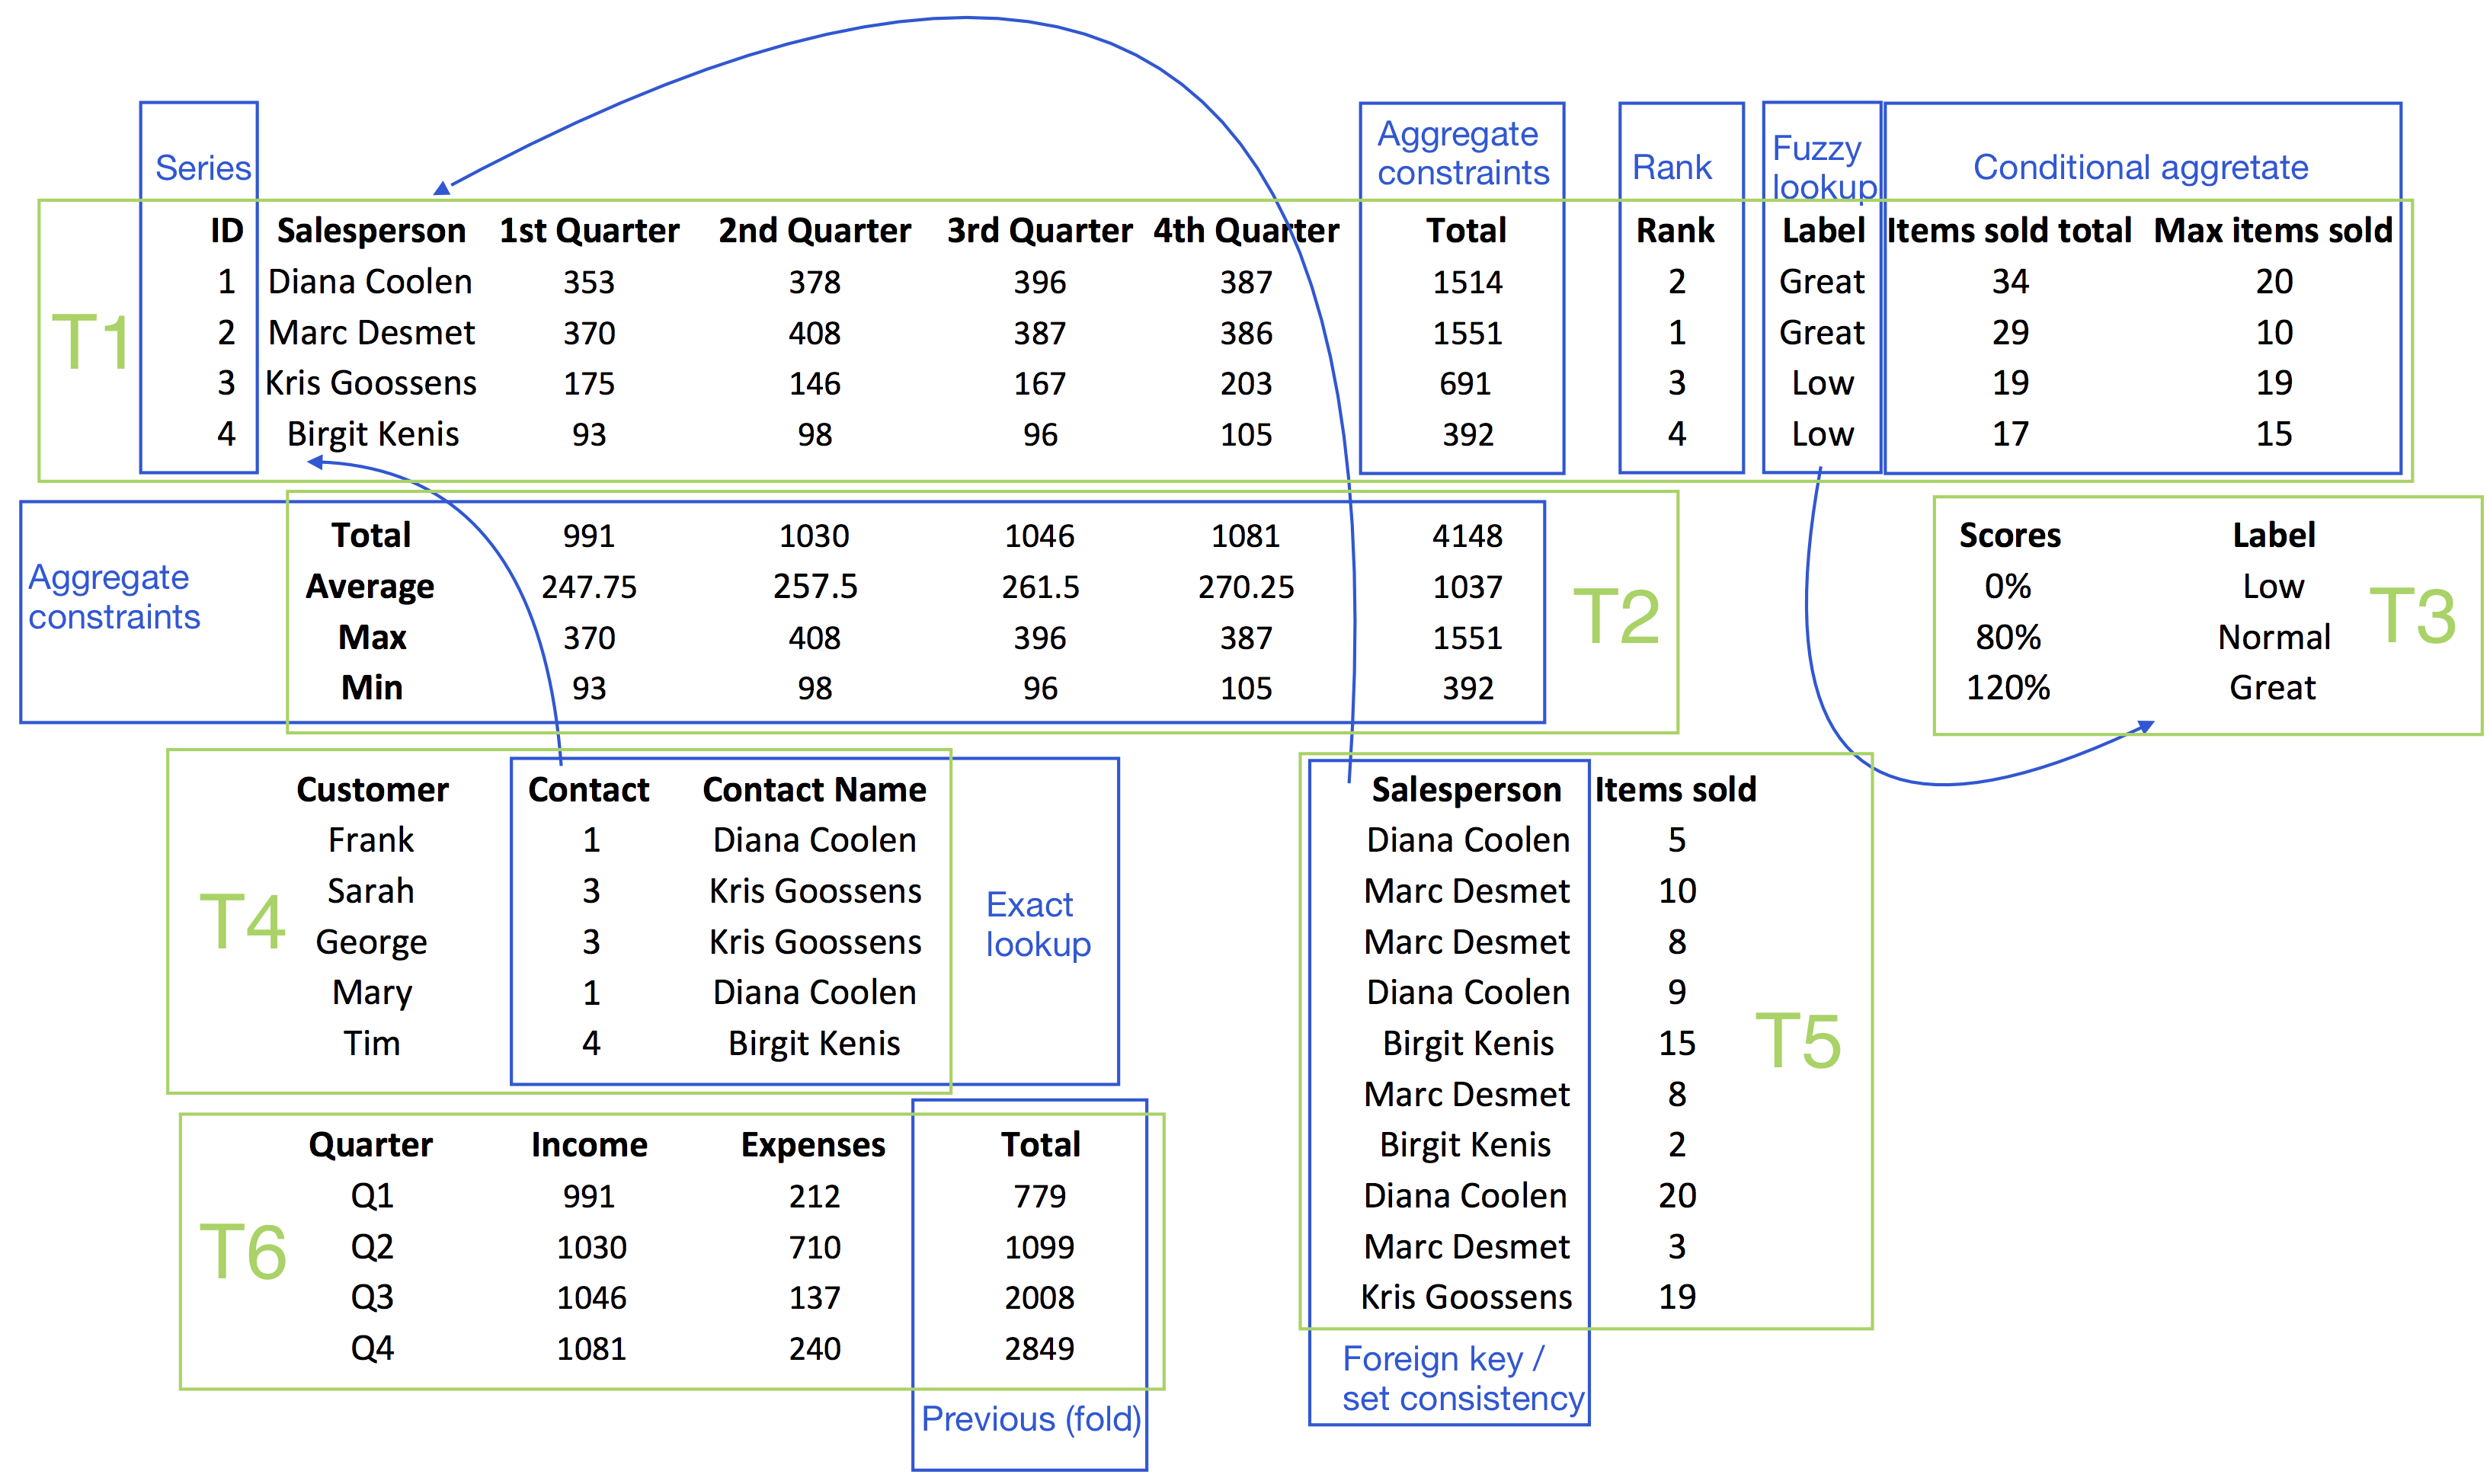
\includegraphics[width=0.75\textwidth]{figures/Demo.png}
  \end{center}
  \vspace{-10pt}
  \caption{Example spreadsheet (black words and numbers only). Blue and green elements are added by us to clarify the relations.}
  \label{fig:main_example}
\end{figure*}

\section{Formalization}\label{sec:formalization}
As we focus on spreadsheet data, we first introduce the general concepts of cells, group and constraint templates, using the (multi-table) sheet in Figure~\ref{fig:main_example} as running example.

\subsection{Cells, vectors and groups}
\tias{perhaps we should not introduce cells, we reason at the level of vectors!}
A spreadsheet may conceptually consist of multiple tables, such as in Figure~\ref{fig:main_example}. We will describe a method of extracting tables from a big spreadsheet in Section~\ref{sec:approach}, however this is not the core of our learning method. Our formalization reasons over tables directly.


Formally, a table is an $n \times m$ matrix. Each entry is called a \textit{cell}.
A cell has a {\em type}, which can be numeric or textual. We further distinguish numeric types in subtypes: integer and float. We also consider \textit{None} as a special type when a cell is empty; \textit{None} is a subtype of all other types.
A set of cells is called \textit{type-consistent} iff all cells in the set are of the same type (\textit{None} is consistent with everything).
%Certain constraints, such as \textit{rank} or \textit{series}, make use of the numeric subtype by requiring its arguments to be integers.

We consider various sets of cells with the following notation:
\begin{itemize}
  \item {\bf Cell}: We use the notation $T[a,b]$ to refer to a particular cell in the table~$T$ at the row with index~$a$ and the column with index~$b$.

  \item {\bf Columns and rows}: For a table $T$, we use notation $T[a,{:}]$ to refer to the $a$-th row, and similarly $T[{:},a]$ for the $a$-th column. % to refer to a subrange from $a$ to $b$ we use $T[a{:}b,]$ ($T[,a{:}b]$).

  \item
  A \textbf{vector} is a type-consistent row or column.
  If a vector is a row (column), we say that it has a \textit{row} (\textit{column}) orientation. The \textit{length} of a vector is the number of cells in that vector.

  \item
  A \textbf{group} is a projection of a matrix onto a set of consecutive rows or columns. %In this work we only consider consecutive rows and columns.
  We use the following notation to refer to a row-oriented group with rows ranging from $a$ to $b$: $G = T[a{:}b,:]$, where $a,b$ are natural numbers. Similarly, we have $G = T[{:},a{:}b]$ for a column-oriented group.
  The vectors in a group have to be type-consistent, consecutive in the original table and of equal length.
  The \textit{size} of a group is the number of vectors in the group, while the \textit{length} of a group is the length of its vectors. 
  %The \textit{length} of a row (column) group $G$, written as \textit{length(G)}, is the number of its columns (rows); We call a group $G$ \textit{numeric} (\textit{textual}, etc), written as \textit{numeric(G)}, if all its vectors contain numeric (textual, etc) elements.

  \item
  A \textbf{subgroup} $G'$ of a group $G$ is simply a projection of $G$ onto a consecutive subset its vectors. % is a subrange of vectors belonging to a group $G$. If the subgroup $g$ must contain only one vector, we write $g \in G$. %It defines what it means for a constraint to be well-formed
%We refer to a subgroup of a group $G$ in \groups as $g$. A \textit{subgroup} $g$ is a subrange of vectors in a group $G$. If a subgroup $g$ must contain only one vector, we write $g \in G$.
% A \textit{subgroup} $G'$ is a subrange of vectors belonging to a group $G$. If the subgroup $\{v\}$ must contain only one vector, we write $v \in G$.
\end{itemize}
%For notational convenience, we will refer to vectors in {\rm roman} and to groups in {\bf bold}. {\bf CHECK}

%When we do not want to distinguish between cells, columns, rows, vectors or groups, we shall talk about a {\em set of cells}.

\paragraph{Example}
Consider Table~1 in Figure~\ref{fig:main_example}, its rows are not type consistent (i.e. they contain both numeric and textual data).
Ignoring the (all-textual) header, Table~1 can be divided into the following five column-oriented groups:
{\small
\begin{align*}
&G_1 = \range{T_1}{\rangeall}{1},
&G_2 = \range{T_1}{\rangeall}{2},\\
&G_3 = \range{T_1}{\rangeall}{\rangeto{3}{8}},
&G_4 = \range{T_1}{\rangeall}{9},\\
&G_5 = \range{T_1}{\rangeall}{\rangeto{10}{11}}.
\end{align*}
}
An example subgroup is $\range{T_1}{\rangeall}{\rangeto{3}{6}} \subset G_3$, which contains the sales numbers of all employees for the four quarters.

\subsection{Constraint templates}
Our method will extract the applicable constraints (including functions) in a set of tables, based on \textit{constraint templates}.
%
A \template is a triple \textit{(\CName, \CSignature, \CFunction)}:
%Let us elaborate on this:
\begin{itemize}
\item
\textit{\CName}  specifies the syntactic form of the constraint $c(G_1, ...,G_n)$, that is, the name of the constraint $c$ together
with $n$ arguments $G_i$. Thus a constraint $c$ is viewed as a relation or predicate of arity $n$ in first order logic. Note that a function $G_r=f(G_1,...,G_n)$ can be represented with the $n+1$-ary predicate $cf(G_r,G_1,...,G_n)$.
% the list of its variables $v_1,\dots,v_n$.  In ILP terminology, it is known as vocabulary.

\item the \textit{\CSignature} defines the properties that the arguments of the predicate must satisfy. That is, the required types of the arguments, together
with possible further restrictions, e.g., on their length. For example, the signature can restrict the types of the arguments to be groups of integers and require that the length of all arguments be equal. In terms of logical and relational learning \cite{luc_book}, such a \CSignature is known as the {\em bias} of the learner, it specifies when the constraint is well-formed.

\item \textit{\CFunction} is the actual definition of the constraint that specifies when the constraint holds. Given an assignments to its arguments, it can be used to verify whether the constraint is satisfied or not. %holds, in practice this will be a function that can be called when
%the arguments are full instantiated to decide whether the constraint is satisfied or not.
In logical and relational learning this is known as the background knowledge, which provides the definition of the predicate.
\end{itemize}
\tias{Requested by Luc: formulate signature and definition as formula?}

\paragraph{Example}
Several example constraints are illustrated in Table \ref{table:constraints}.  For example, the constraint template \textit{rank} has
\begin{itemize}
  \item \CName: \ecrank{G_r}{G_x}, where $G_r$ and $G_x$ are the arguments;
\item \CSignature: the two arguments $G_r$ and $G_x$ must be numeric groups and of size one; furthermore, the group $G_r$ must be integer (the rank) and the length of groups $G_x$ and $G_r$ must be identical, i.e., $\plength(G_r) = \plength(G_x)$;
\item \CFunction: \ecrank{G_r}{G_x}, whenever each value of $G_r$ is the rank of the corresponding value in $G_x$.
% is satisfied in the mapping $\{ v_x \mapsto g_x, v_y \mapsto g_y \}$ satisfies the constraint iff $g_x \in G_x, g_y \in G_y$ ($G_x \in \groups, G_y \in \groups$) and each value in $g_y$ is the rank of the corresponding value in $g_x$ (possibly with ties).
\end{itemize}
When looking into constraints like $\ecrank{G_r}{G_x}$, it is helpful to see the analogy with both first order logic (FOL) and with constraint satisfaction problems.
From a FOL perspective, the name of the constraint (\textit{RANK}) is just the predicate, and the arguments $B$ and $A$ are the terms, which can be seen as either uninstantiated variables or as concrete values.

This also holds in our setting, where an instantiation of a variable corresponds to a concrete set of vectors (a subgroup). For example for $\ecrank{G_r}{G_x}$ and the spreadsheet in Figure~\ref{fig:main_example}, when we write $\ecrank{\range{T_1}{\rangeall}{8}}{\range{T_1}{\rangeall}{7}}$, then the value of $G_r$ is the $8$th vector in $T_1$: $G_r = \range{T_1}{\rangeall}{8} = \{[2,1,3,4]\}$ and the value of $G_x$ is the $7$th vector: $G_x = \range{T_1}{\rangeall}{7} = \{[1514, 1551, 691, 392]\}$.
\tias{not OK to use set because of column-wise sum? we must properly define it then...}

\newcommand{\sigc}{\ensuremath{\format{Sig}_c}}
\newcommand{\defc}{\ensuremath{\format{Def}_c}}

With this interpretation, we can speak about the signature and definition of a constraint template being satisfied. We say that a signature (definition) of a constraint template with $n$ arguments is satisfied by an assignment $(G_1, ..., G_n)$ if $\sigc(G_1, ..., G_n)$ (respectively $\defc(G_1, ..., G_n)$) is satisfied. Likewise, an assignment $(G_1, ..., G_n)$ satisfies a constraint template $s$ iff $|(G_1, ..., G_n)| = n_s \wedge \sigc(G_1, ..., G_n) \wedge \defc(G_1, ..., G_n)$.

\tias{Luc will probably prefer: $c(A_1, ..., A_n) :- Sig_c(A_1, ..., A_n) \wedge Def_c(A_1, ..., A_n)$ where '$c$' is abused to be both the constraint name and the template}.


%\sergey{moved from the formalization BEGIN}
%l 1) a set of cells, and 2) a set of constraints over those cells.  Notice that the constraints specify the types (or the domains) that one encounters in traditional CSPs.  Notice also, that as in traditional CSPs, the CSP problem defines the variables (the cells) of the problem as well as the constraint that should hold amongst them. The task of CSP-solvers is then to find an assignment to the variables that satisfies all the constraints.  The distinction between variables (cells) and their assignments (their values) is important here.  So, when we speak about cells, vectors and groups, we refer to the variables; when we talk about values, assignments or instances, we refer to the values these cells take in a particular "instantiated" table.

\section{Problem Statement}\label{sec:problem_statement}
The problem of learning constraints from tabular data can be seen as an inverse {\em constraint satisfaction problem} (CSP). A CSP consists of a set of constraints and the
task is to find assignments of values to the variables in the CSP so that all constraints are satisfied.
In the context of spreadsheets where variables could represent cells in tables, solving a corresponding CSP problem would mean completing the tables so that all constraints of the spreadsheet are satisfied.

The inverse problem is, given an assignment to all cells, to find the constraints that are satisfied in the spreadsheet.
We define the {\bf Tabular Constraint Learning Problem} as follows:
%
\begin{definition} \textit{Tabular Constraint Learning.}\label{def:problem_statement}\\
{\bf   Given} ${\cal G}$ a set of groups over fully instantiated tables ${\cal T}$ (all cells have values) and a set of {\template}s ${\cal S}$: {\bf find } all constraints $c_s(G'_1, ..., G'_n)$ that match the syntax of a \template~$s \in {\cal S}$ and where all subgroups $G'_i \subseteq G_i$ with $G_i \in {\cal G}$, satisfy both the signature and the definition of that \template.
\end{definition}
% Let us now define what it means for a constraint from \template to hold in general. Let $t$ be a \template, $S$ be a mapping from variables to the subgroups of \groups, and $C$ be the constraint $t^S$, then $C$ \textit{holds} iff all constraints in $\text{\CSignature}^S$ and $\text{\CFunction}^S$ of $C$ hold.
% \sergey{moved from formalization END}

%Here we formalize the statement in terms of \template and group assignments as follows:
%   \begin{tabular}{ll}
%     \multicolumn{2}{l}{{\textbf{Tabular Constraint Learning Problem}}}\\
%     \textbf{Given:}& the set of all groups $\groups$ and of \template $\constraints$\\
%     \textbf{Find:}&  all constraints $C$ over \groups for each template $t$ in \constraints \\
%   \end{tabular}

An example solution for the type-consistent groups of the tables in Figure~\ref{fig:main_example} and {\template}'s in Table~\ref{table:constraints} is shown in Figure~\ref{fig:sol_example}.


Depending on the application, a solution to the tabular constraint learning problem may contain \textit{redundant} constraints, cf. \cite{luc_book}. This is because constraints may be logically equivalent or may be implied by other constraints.

More formally, a constraint $c_1(G_1, ... G_n)$ \textit{implies} another constraint~$c_2(G'_1, ..., G'_m)$ whenever
the  following statement holds: $$\forall G_i, G'_j : c_1(G_1, ... G_n) \rightarrow c_2(G'_1, ... G'_m).$$

We shall only consider {\em range-restricted} implications, that is, we shall require that $\{G'_1, ..., G'_m\} \subseteq \{G_1, ..., G_n\}$.
To simplify notation, and in line with logic programming, we shall often make the quantification implicit and simply write this as rules $ c_1(G_1, ... G_n) \rightarrow c_2(G'_1, ... G'_m)$.  We say that the first constraint is more specific than the second, and the second is more general.


% where the second one ranges over a subsets of the arguments of the first, iff whenever the first constraint is true, the second must also be true. More formally, $\forall G'_1, ..., G'_n$ s.t. $\{G''_1, ..., G''_m\} \subseteq \{G'_1, ..., G'_n\},\, c_1(G'_1, ... G'_n) \rightarrow c_2(G''_1, ..., G''_m)$ll.

\paragraph{Example}
Consider the following implication:
$$\ecperm{G} \rightarrow \ecalldiff{G}$$
(it can be seen in Table~\ref{table:constraints} that both constraints only hold if $G$ is a vector).
In this case the arguments are identical in both constraints.
Given that the problem is to find the set of {\em all} constraints, and that the more general constraint is entailed
by the more specific one, the $ALLDDIFFERENT(G)$ constraint will be {\em redundant}.
So, for most applications, it will be sufficient to output only the most specific one.

A more involved example is
$$\eclookup{G'_2}{G'_1}{H'_1}{H'_2} \rightarrow \ecfkey{G'_1}{H'_1}$$
which states
that a look-up constraint implies a foreign-key constraint. In the look-up constraint $\eclookup{G'_2}{G'_1}{H'_1}{H'_2}$ the values in the vector $G'_2$ are determined by looking up the corresponding value in vector $G'_1$ in vector $H'_1$ and returning the corresponding value in vector $H'_2$. In Figure~\ref{fig:main_example} we have $\eclookup{\range{T_{4}}{\rangeall}{3}}{\range{T_{4}}{\rangeall}{2}}{\range{T_{1}}{\rangeall}{1}}{\range{T_{1}}{\rangeall}{2}}$. This implies a foreign-key constraint $\ecfkey{G'_1}{H'_1}$ where each of the values in vector $G'_1$ must appear in $H'_1$ for the look-up to work.

Two constraints are \textit{equivalent} if they imply one another. %More formally, $\forall G'_1, ..., G'_n$ s.t. $\{G''_1, ..., G''_n\} = \{G'_1, ..., G'_n\},\, c_1(G'_1, ... G'_n) \leftrightarrow c_2(G''_1, ..., G''_n)$.
An example within the same \template is for the sum over vectors constraint: $G_1 = +(G_2, G_3) \leftrightarrow G_1 = +(G_3, G_2)$. A related example over multiple constraints is $G_1 = +(G_2, G_3) \leftrightarrow G_1 = \textit{SUM}(H)$ with $\textit{size}(H) = 2$ and $G_2 \subset H, G_3 \subset H$.
\luc{Do we really need this, or can we write it in a real equivalence --- conjunctive formula?}

A good way to deal with equivalent constraints is to work with a \textit{canonical} constraint among the equivalent ones. For example, for equivalent constraints of the same \template, this could be the constraint where the groups are ordered by table, orientation and row/column identifier. For equivalent constraints of different templates one could define heuristics such as that some templates are preferred over others, e.g. binary sum over n-ary sum, sum over difference, etc.

Because dealing with redundancy is often application-dependent, we explain in the next section our generic method for finding all constraints.

\tias{I am not defining a new problem for 'most specific canonical tabular constraint learning' because we loosely showed how implications and equivalences would be expressed, but not how to express canonicity and we did not claim that most specific is always best.}
\tias{Note also that our method finds ALL constraints; it uses specificity to faster traverse the search space, but the resulting set of constraints found would be the same, whether or not using the specificity (see 4.2.1).}

%Let us introduce the version of tabular constraint learning by modifying Definition \ref{def:problem_statement} that takes into account the specificity relation between constraint templates.
%
%\begin{definition} \textit{Condensed Tabular Constraint Learning}\label{def:condensed_problem_statement}\\
%  Given a set of instantiated tables~${\cal T}$ (all cells have values), a set of {\template}s~${\cal S}$, a set of groups~${\cal G}$ over the tables~${\cal T}$, and the set of all specifity rules~\dependencies: find the set of all constraints $s(G_1', ..., G_n')$ that are satisfied  in ${\cal T}$, for which all $G_i' \subseteq G_i \in {\cal G}$, the (sub)groups $G_1', ... , G_n'$ satisfy the signature of the constraint template~$s \in {\cal C}$ and there is no $s'$ in ${\cal C}$ such that $s'(G_h',\dots,G_k')$ holds (for $1 \leq h \leq k \leq n$) and  $s'$ is more specific than $s$ in \dependencies.
%\end{definition}

% \begin{minipage}[c]{14em}
%   \vspace{5pt}
%   \begin{tabular}{ll}
%     \multicolumn{2}{l}{{\textbf{Condensed Tabular Constraint Learning Problem}}}\\
%     \vspace{-4pt}
%     &\\
%     \textbf{Given:}& the set of all groups $\groups$ and of \template's $\constraints$,\\
%     & a constraint specificity DAG \dependencies \\
%     \textbf{Find:}& all the most specific wrt \dependencies constraints $C$ over \groups\\
%     & for each $t$ in \constraints \\
%   \end{tabular}
%   \vspace{6pt}
% \end{minipage}

%This version explicitly takes into account the specificity of the constraints and invalidates some of the solutions that are entailed by the tabular other solutions.

\newcommand{\tcl}{Tabular Constraint Learning}
%\newcommand{\ctl}{Condensed Tabular Constraint Learning}
\section{Approach to Tabular Constraint Learning}\label{sec:approach}
This section describes our approach to \tcl. The main method takes \textit{groups} and {\template}s as input, and is described in Section~\ref{sec:algo}. We first explain how tables and groups can be extracted from raw spreadsheet data.

\subsection{Table and group detection} \label{sec:make_groups}
%A spreadsheet may contain multiple tables, and a table in turn will contain multiple (type-consistent) groups.
Many spreadsheets contain headers that provide hints at where the table(s) in the sheet are and what the meaning of the rows and columns is. However, detecting tables and headers is a complex problem on its own~\cite{header}. Furthermore, headers may be missing and their use often requires incorporating language-specific vocabulary, e.g. in English.

%\tias{0. preprocess: currencies and precentual to numeric, 1. tables from spreadsheets, 2. groups from tables. Ext: could be done interactively.}
Fully automatic table and header detection is not the core of our work. We hence built a visual tool that uses a simple method to detect tables in the data and allows a user to correct these.

The way the table detection in the tool works is as follows:
First, we preprocess the spreadsheets so that currency values are transformed into their integer or float value and percentual data is transformed into the corresponding floating point representation (e.g. $85\%$ as $0.85$).
Next, every row in the spreadsheet is partitioned into blocks of columns that are separate by at least one $None$ value. Then, the blocks in each row are greedily merged to obtain rectangles. Finally headers are removed by checking whether the first row or column is all textual while the next row or column is not; in that case the assumed header is removed.

It should be clear this simple method only works if all tables are clearly separated by $None$ values and that headers of fully textual tables are not detected, among other things. Hence, in the visual tool the user can correct the detected tables if needed. \tias{I think it would be good if we could show a screenshot of this tool...}

From each table, row-oriented and column-oriented groups are then extracted by partitioning the rows (columns) into type-consistent parts. This step can also be verified by a user in the visual tool.

From here on we will assume that groups and tables are given.

\newcommand{\temps}{\ensuremath{S}}
\subsection{Algorithm} \label{sec:algo}
Our method solves the \tcl problem by checking for each template what combination of groups can satisfy the signature, and which specific subgroups satisfy the definition.

The main challenge is to avoid having to check each possible combination of group and subgroup on each constraint template, as well as developing an \textit{extensible} method in which new constraint templates can be plugged in with relative ease. %We will use constraint satisfaction technology to partly answer this challenge.
To answer this challenge we separate checking the signature of a constraint template from checking the definition of a constraint template. Furthermore, we use constraint satisfaction technology to jointly search for and test the signature over all group combinations.

The pseudo-code of the main method is shown in Algorithm~\ref{algo:tcl}; it consists of three key components: 1) templates can depend on each other, so they are ordered to avoid having to verify the same template multiple times; 2) we generate all combinations of groups that can satisfy the signature using constraint satisfaction techniques; 3) from this, all satisfying subgroups are generated.

\begin{algorithm}[t]
  \begin{algorithmic}
    \footnotesize
    \State \textbf{Input:} $\groups$ -- groups, $\constraints$ -- \template's, \dependencies -- dependency graph
    \State \textbf{Output:} $C$ -- learned constraints
    \State $C \gets \emptyset$ %\Comment{The set of constraints}
  \ForAll{$t \in \constrainttorder(\constraints,\dependencies)$}
  \State $n \gets$ number of arguments of constraint $c_t$
    \ForAll{$(G_1, \dots, G_n) \in \generategroups(t, \groups, C)$}
      \State $C \gets C \cup \findassignment(t, (G_1, \dots, G_n))$
    \EndFor
  \EndFor\\
\Return $C$
\end{algorithmic}
\caption{Tabular constraint learning}
\label{algo:tcl}
\end{algorithm}

%First, constraint templates are ordered such that they can be treated sequentially and each only once.
%Then, for each constraint template~$s \in \temps$ we generate a set~$A$ of \textit{group-assignments} that satisfy the \CSignature of~$s$.
%Every group assignment assigns a group~$G \in \groups$ to every argument of the template.
%In the third step, for every assignments $(G_1, ..., G_n) \in A$ we find all constraints $s(G_1', ... G_n')$ that hold on the data (satisfy the \CFunction), such that every subgroup $G_i' \subseteq G_i$.

%Our Algorithm \ref{algo:tcl} is in line with the ``generate-and-test'' paradigm that is well-known in AI \cite{whaisasp}, however, we apply the approach on two levels, generating and testing groups according to their properties and generating and testing subgroups on the actual data.
%We will explain and illustrate the three key steps in detail.

We now describe each of the three components in more detail.

\subsubsection{Template ordering}
As discussed before, a constraint may imply another constraint. This is apparent when looking at the template signatures in Table~\ref{table:constraints}, where one can see that some signatures depend on other constraints, such as $LOOKUP$ depending on $FOREIGNKEY$.

In Inductive Logic Programming, one often exploits implications between constraints to structure the search space \cite{luc_book}.
In our method, we use these dependencies/implications to define a dependency graph between the templates. We assume the signatures do not contain equivalences or loops, and hence the resulting graph is a directed acyclic graph (DAG).
Figure~\ref{fig:learning_order} shows the dependency graph extracted from the signature definitions in Table~\ref{table:constraints}. 
Constraint templates that have no dependencies are omitted. 

\begin{figure}[t]
  \centering
  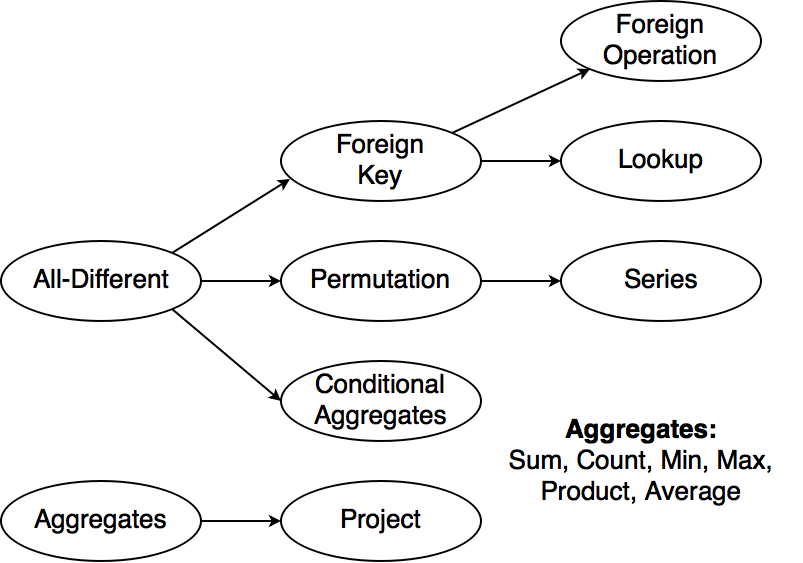
\includegraphics[width=0.8\linewidth]{figures/constraint_dependency.png}
  \caption{Dependency graph; an arrow from~$s_1$ to~$s_2$ indicates that $s_1$ is implied by $s_2$ because the \CSignature of~$s_2$ depends on $s_1$ to hold on a specific subset of $s_2$ its groups.
    The graph is extracted from the Signature column in Table \ref{table:constraints}.
  }
  \label{fig:learning_order}
\end{figure}

The $\constrainttorder(\constraints,\dependencies)$ module in our method takes a set of {\template}s and a DAG as input and produces a linear ordering of the templates such that the more general, implied constraint templates (the requirements) are ordered before the templates that depend on them.

\paragraph{Example}
As mentioned before, $\eclookup{G'_2}{G'_1}{H'_1}{H'_2}$ implies $\ecfkey{G'_1}{H'_1}$ and hence the $LOOKUP$ constraint template depends on $FOREIGNKEY$ in Figure~\ref{fig:learning_order} and will be earlier in the ordering.

% not helpful:
%The \ecrank{v_y}{v_x} constraint does not have any dependencies, however in a restricted version without ties, groups assigned to $v_y$ would always be a permutation of numbers $1, 2, ..., \textit{length}(v_y)$.

\subsubsection{Candidate group generation}
%The goal of this step is to prune out impossible groups from the beginning by looking at their properties rather than their actual content (\CSignature vs \CFunction).
Given a constraint template and the set of all groups ${\cal G}$, the goal is to find all combinations of groups that satisfy the constraint signature. Let there be $n$ groups and let the constraint have $k$ arguments, then a simple generate-and-test method would have to test $\tbinom{n+k-1}{k}$ combinations (given that groups can be repeated), which grows very rapidly with $n$.

However, the properties defined in the signature, such as related to type or size, can be used to avoid considering certain groups for certain arguments. Furthermore, the choice of one argument can influence the possible candidates for the arguments, for example if they must have the same length. Instead of writing specialized code for each of these cases, we make use of the built-in reasoning mechanisms of constraint satisfaction solvers.

%Finding candidate groups for a \template~$t$ can be seen as a Constraint Satisfaction Problem (CSP) dependent on the \CSignature of~$t$.
%For every argument in~$t$ we consider all groups~\groups (or all candidates from a more general constraint) and prune these candidate groups using their types and other requirements imposed by the templates \CSignature, such that a group~$G \in \groups$ is selected if there is at least one subgroup~$G' \subseteq G$ that satisfies the \CSignature.

A Constraint Satisfaction Problem (CSP) is a triple $(V,D,C)$ where $V$ is a set of \textit{variables}, $D$ the domain of possible values each variable can take and $C$ the set of constraints over $V$ that must be satisfied. In our case, we define one variable $V_i$ for each argument of the constraint. Each variable can be assigned to each of the groups in ${\cal G}$, so the domain consists of $|\{\cal G\}|$ identifiers.

To reason over the groups, we automatically add to the constraint program a set of background facts that contain the properties of each group, namely its type, size and length. We also add all previously found constraints of constraint templates that are implied by this template. The actual constraints then express the properties defined in the signature, such as whether arguments are of a certain type, have certain dependencies or have to be equal length or orientation, etc.
\tias{More detailed description of the properties commented out, feel free to put in}
%Translation:
%\begin{description}
%  \item[Type] Require group that has supertype (e.g. integer => require numeric group, because subgroup might be integer)
%  \item[Length] Require group to have exact length (subgroups have the same length)
%  \item[Vectors / columns / rows] Require group to have at least the amount of vectors, columns, rows required
%  \item[Dependency] Fix dependent variables, for every assignment construct CSP that attempts to find values for the other variables
%  \item[Same length / table / orientation] Require groups to gave the same length table ...
%\end{description}

% TODO: old text, rephrase a bit
Constraints derived from the signature can usually but not always be enforced exactly on a group, as we have to consider whether subgroups could satisfy them.
For example, the \CSignature of ?? requires $v_r$ to be integer.
If a numeric group is assigned to $v_r$ then some subgroups may have type float while other may be of type integer, therefore, this group cannot be discarded.


\paragraph{Example}
We show this construction of a CSP for the constraint template $\ecsumprod{G'}{H'}{I'}$ in Table~\ref{table:constraints}. It defines that $G'$ is a cell whose values is the result of the sum of products of rows in $H'$ and columns in $I'$.
%
There are three \textit{variables} $X, Y, Z$ corresponding to group $G'$, $H'$ and $I'$ respectively. The domains are $D(X) = D(Y) = D(Z) = \{1, \ldots, |{\cal G}|\}$. Finally, the constraints are:
\begin{align*}
&numeric(X) \land numeric(Y) \land numeric(Z) \\
&\pcols(X) = 1 \land \prows(X) = 1 \\
&\plength(Y) = \plength(Z) \land \plength(Y) \geq 2
\end{align*}
\tias{Sumproduct is a rather peculiar constraint for spreadsheets... perhaps switch to one with a dependency, e.g. look-up?}
\sergey{ok, we need to see if look-up would fit here}
\\\\


The $\generategroups(\textit{t,{\cal G},C})$ method will construct this CSP and query a solver for all satisfying solutions. This is the required result set.

\subsubsection{Constraints over satisfying subgroups} \label{sec:algo:subgr}
In the previous step, $\generategroups(\textit{t,{\cal G},C})$ generates tuples of candidate groups $(G_1, ..., G_n)$ for the constraint template $t$ with $n$ arguments. In this step, $\findassignment(t, (G_1, \dots, G_n))$, the goal is to enumerate the subgroups $(G'_1, ..., G'_n), \forall i, G'_i \subseteq G_i$ that satisfy both the signature and the definition of the constraint template $t$. The main difference with the previous step is that the group generation reasons about the \textit{properties} of the groups (type, size, length, ...), while this step reasons about the actual \textit{content} of the vectors in the groups, that is, the data.

\paragraph{Example}
Consider the sum-over-rows constraint template $\ecsumr{\sg_r}{\mathbf{\sg_x}}$. In the group generation, all numeric groups where the length of $\sg_r$ vector is equal to the number of rows in $\mathbf{\sg_x}$ has been enumerated. An example from Table~\ref{table:constraints} is $(\sg_r, \mathbf{\sg_x}) = (T_1[:,3:8],T_1[:,3:8])$. Note that this does not match the signature exactly yet: $\sg_r$ contains more than one vector. We can now generate all vectors in $T_1[:,3:8]$ for $\sg_r$ and all subgroups of $T_1[:,3:8]$ for $\mathbf{\sg_x}$ and test whether $\forall i, \sg_r[0][i] = \sum_j \mathbf{\sg_x}[j][i]$ where $G[j][i]$ indicates the $i$the value of the $j$th vector in $G$. An example solution is $(T_1[:7], T_1[:,3:6])$.
\\\\

One can formulate this as a constraint satisfaction problem, similar to what we did in the previous section, or use a simple generate-and-test approach. In contrast to the previous step, the number of subgroups to generate here are typically manageable: $O(n*m^2)$ with $m$ the number of vectors in the largest group; we only consider continuous ranges in subgroups, so a subgroup of size $m$ has $m*(m+1)/2$ possible subgroups to consider. Furthermore, few constraint solvers support floating point numbers, which are prevalent in spreadsheet.

For this reason, our current implementation uses a simple generate-and-test method that takes the required size/length of the groups into account, and sequentially verifies whether the elements of the vectors satisfy the definition. The pseudo-code for this approach is shown in ...\tias{Add pseudocode!!}

\begin{verbatim}
VERY PSEUDOcode:
something recursive that handles vectors/subgroups differently like this?
check(Groups, X, Test):
  if |Groups| == 0:
    forall i in ?: vector elements...
      if not Test(X):
        return []
    return X
  // else
  all = []
  Group = Groups.pop(0)
  if vector(Group):
    forall Vec in Group:
      all += check(Groups, X + Vec, Test)
  else:
    forall Subgroup in Group:
      all += check(Groups, X + Subgroup, Test)
  return all
\end{verbatim}

Note that for some constraint definitions, there are \textit{symmetries} over the arguments that lead to trivially equivalent solutions, for example $G_1 = +(G_2, G_3) \leftrightarrow G_1 = +(G_3, G_2)$. \tias{How are they stopped in the code? should be part of the pseud-code because not part of $Test(X)$?}

\paragraph{Example 2, not used (should be replaced by pseudo-code above?)}
Sum Product

Implementation: finds subgroups based on assignments\\
Method $Test(G_R, G_{O_1}, G_{O_2})$\\
$If \lnot G_{O_1} < G_{O_2}: Reject~\#~Canonicity$\tias{ill-defined, $G_{O_1}$ is a group and $<$ not defined on it (on vector identifiers rather than content?)}\\
$If data(G_R) = data(G_{O_1}) \bullet data(G_{O_2}): Accept$ \tias{does not show that reasons over content of vectors}
\\\\
Method $FindSubgroups(Assignments)$\\
$Return \{ (G_R', G_{O_1}', G_{O_2}') | \exists (G_R, G_{O_1}, G_{O_2}) \in Assignments \land G_R' \subseteq G_R \land G_{O_1}' \subseteq G_{O_1} \land G_{O_2}' \subseteq G_{O_2} \land Test(G_R', G_{O_1}', G_{O_2}') \}$ \tias{does not enforce size of subgroups (e.g. vectors)?}


\subsection{Implementation}
We provide some more details of our implementation of the above algorithmic approach, to ease reproducibility.

\paragraph{Constraint solvers}
Generic constraint solving technology can be used for the candidate group generation as well as for enumerating the satisfying subgroups. Constraint solvers can be categorized as being stand-alone solvers, meaning that they have a text-based modeling language in which the CSP must be formulated, and \textit{embedded}, meaning that they have a programmatic API to formulate the CSP.

Our implementation supports the ASP \cite{whaisasp} formalism, using the stand-alone Clingo 4.5.4 \cite{clingo} solver, the stand-alone Constraint Programming language MiniZinc \cite{minizinc} with the Gecode 4.4.0 solver which supports floats, as well as an embedded Python-based CP solver \cite{python_constraint}. The constraint signature that must be satisfied to generate the groups can be specified in each of the tree formalisms, to ease prototyping and extendability towards new constraints. The embedded solver is fastest as it does not have the overhead of file-writing and calling an external program, and is used in the experiments below.

\paragraph{Redundancy}
There are only types of redundancy that we eliminate during search. The first is the removal of symmetric attribute assignments as explained in Section~\ref{sec:algo:subgr}.

The second is that there be \textit{overlapping} subgroups that satisfy the definition, such as \tias{There is no example in the example figure? I was thinking of max/min, but it is over the entire vector always...}.
In this case we chose to omit those subgroups that are fully contained within a larger subgroup since this can lead to over-fitting.

\paragraph{Constraints}
The constraints that are currently supported in our system are shown in Table~\ref{table:constraints}. All these constraints are available in popular spreadsheet software, except the first two constraints (alldifferent and permutation). These two constraints are \textit{structural} constraints, which we added so they can be used in the signature of other constraint templates; they are also popular constraints in constraint satisfaction~\cite{modelseeker}.

%Their dependencies are reflected in their \CSignature and shown in Figure~\ref{fig:learning_order}.
%These constraints have been selected based on the most-used Excel functions as well as their occurrence in various example spreadsheets we observed.

Note that \samuel{Motivate why product, not sum (=diff) you only need one, hardcoded preference for display - diff not present - pruning relation?} 

\tias{Not used, should be cut!?:}
Generally \CSignature and / or the \CFunction can be relaxed to capture more constraints in the data, however, this also comes at a performance penalty. \samuel{More on this / example?} \tias{Yes, either explain in detail or cut}

\begin{table*}
\caption{Overview of constraint templates implemented in our system, which covers the most popular spreadsheet constraints we encountered. The templates marked with $\dagger$ are aggregate constraint templates, the table shows the version for sum but the implementation also supports max, min, average, product and count. Subgroups in normal font have to be vectors, while subgroups in bold may contain more than one vector.\label{table:constraints}}
  {\centering
  \begin{tabularx}{\textwidth}{l X X}
    \textbf{\CName} & \textbf{\CSignature} & \textbf{\CFunction}\\ \hline \hline
    $\ecalldiff{\sg_x}$
      & $\discrete(\sg_x)$
      & All values in $\sg_x$ are different: $\sg_x[i] \neq \sg_x[j]$ if $i \neq j$
      \\ \hline
    %X = Y & & \\
    $\ecperm{\sg_x}$
      & $\numeric(\sg_{x})$, $\ecalldiff{\sg_{x}}$
      & The values in $\sg_{x}$ are a permutation of the numbers $1$ through $\plength(\sg_{x})$.
      \\ \hline
    \ecseries{\sg_x}
      & $\numeric(\sg_{x})$ and $\ecperm{\sg_{x}}$
      & $\sg_{x}[1] = 1$ and $\sg_{x}[i] = \sg_{x}[i - 1] + 1$.
      \\ \hline
    \ecfkey{\sg_{fk}}{\sg_{pk}} & $\sg_{fk}$ and~$\sg_{pk}$ are both $\discrete$; $\ptype(\sg_{fk}) = \ptype(\sg_{pk})$; $\ptable(\sg_{fk}) \neq \ptable(\sg_{pk})$; and $\ecalldiff{\sg_{pk}}$ & Every value in~$\sg_{fk}$ also exist in~$\sg_{pk}$ \\ \hline
    % TODO check out
    \eclookup{\sg_r}{\sg_{fk}}{\sg_{pk}}{\sg_{val}}
      & $\sg_{fk}$ and $\sg_{pk}$ are both $\discrete$; arguments $\{\sg_{fk}, \sg_{r}\}$ and $\{\sg_{pk}, \sg_{val}\}$ within the same set have the same \plength, \ptable and \por; $\sg_{r}$ and~$\sg_{val}$ have the same type; and \ecfkey{\sg_{fk}}{\sg_{pk}}.
      & $\sg_r[i]$ is the same value as looking up~$\sg_{fk}[i]$ in~$\sg_{pk}$  and returning the corresponding value in~$\sg_{val}$.
      \\ \hline
    \eclookupfuzzy{\sg_r}{\sg_{fk}}{\sg_{pk}}{\sg_{val}}
      & \textit{Same as lookup}
      & $\sg_r[i]$ is the same value as looking up the last item in~$\sg_{pk}$ smaller than~$\sg_{fk}[i]$ and returning the corresponding value in~$\sg_{val}$.
      \\ \hline
    \eclookupprod{\sg_r}{\sg_1}{\sg_{fk}}{\sg_{pk}}{\sg_{val}}
      & Arguments $\{\sg_{r}, \sg_{1}, \sg_{fk}\}$ are $\numeric$, arguments $\{\sg_{pk}, \sg_{val}\}$ are $\discrete$ and within both sets all arguments have the same \plength, \ptable and \por; also \ecfkey{\sg_{fk}}{\sg_{pk}}.
      & $\sg_{r}[i]$ is the obtained by multiplying $\sg_{1}[i]$ with $\eclookupf{\sg_{fk}}{\sg_{pk}}{\sg_{val}}{}[i]$.
      \\ \hline
    \ecprod{\sg_r}{\sg_1}{\sg_2}
      & Arguments $\{\sg_{r}, \sg_{1}, \sg_{2}\}$ are all $\numeric$ and have the same $\plength$
      & $\sg_{r}[i] = \sg_{1}[i] \times \sg_{2}[i]$.
      \\ \hline
    \ecdiff{\sg_r}{\sg_1}{\sg_2}
      & Arguments $\{\sg_{r}, \sg_{1}, \sg_{2}\}$ are all $\numeric$ and have the same $\plength$ and $ \por$
      & $\sg_{r}[i] = \sg_{1}[i] - \sg_{2}[i]$.
      \\ \hline
    \ecproj{\sg_r}{\mathbf{\sg_x}}
      & Arguments $\{\sg_{r}, \mathbf{\sg_x}\}$ all have the same $\plength$, $\por$, $\ptable$ and $\ptype$; $\mathbf{\sg_x}$ contains at least~2 vectors; and $\sg_r = \mathit{SUM}(\mathbf{\sg_x}, \por(\mathbf{\sg_x}))$
      & At every position~$i$ in $1$ through $\plength(\sg_{r})$ there is exactly one vector~$v$ in $\mathbf{\sg_x}$ such that $v[i]$ is a non-blank value, then $v[i] = \sg_{r}[i]$.
      \\ \hline
    \ecrank{\sg_r}{\sg_x}
      & $\integer(\sg_{r})$; $\numeric(\sg_{x})$; and $\plength(\sg_{r}) = \plength(\sg_{x})$
      & The values in $\sg_{r}$ represent the rank (from largest to smallest) of the values in $\sg_{x}$ (including ties)
      \\ \hline
    \ectotal{\sg_r}{\sg_{pos}}{\sg_{neg}}
      & Arguments $\{\sg_{r}, \sg_{pos}, \sg_{neg}\}$ are all $\numeric$ and all have the same $\plength$, which is at least $2$
      & The values in $\sg_{r}$ are a running total, each value $\sg_{r}[i] = \sg_{r}[i - 1] + \sg_{pos}[i] - \sg_{neg}[i]$.
      \\ \hline
    $\ecsumc{\sg_r}{\mathbf{\sg_x}}^\dagger$
      & $\sg_r$ and $\mathbf{\sg_x}$ are $\numeric$; $\prows(\mathbf{\sg_x}) \geq 2$; and $\pcols(\mathbf{\sg_x}) = \plength(\sg_r)$
      & Each value in $\sg_{r}$ is obtained by summing over the corresponding column in $\mathbf{\sg_x}$.
      \\ \hline
    $\ecsumr{\sg_r}{\mathbf{\sg_x}}^\dagger$
      & $\sg_r$ and $\mathbf{\sg_x}$ are $\numeric$; $\pcols(\mathbf{\sg_x}) \geq 2$; and $\prows(\mathbf{\sg_x}) = \plength(\sg_r)$
      & Each value in $\sg_{r}$ is obtained by summing over the corresponding row in $\mathbf{\sg_x}$.
      \\ \hline
    $\ecsumif{\sg_r}{\sg_{fk}}{\sg_{pk}}{\sg_{val}}^\dagger$
      & $\sg_{fk}, \sg_{pk}$ are $\discrete$; $\sg_{r}, \sg_{val}$ are $\numeric$; within the sets $\{\sg_{val}, \sg_{fk}\}$ and $\{\sg_{pk}, \sg_{r}\}$ arguments have the same $\plength$ and $\por$; $\sg_{fk}$ and $\sg_{val}$ have the same $\ptable$; $\sg_{fk}$ and $\sg_{pk}$ must have different $\ptable$s but the same $\ptype$; and \ecalldiff{\sg_{pk}}
      & The value for $\sg_{r}[i]$ is obtained by summing all values $\sg_{val}[j]$ where $\sg_{fk}[j] = \sg_{pk}[i]$
      \\ \hline
    \ecsumprod{\sg_r}{\sg_1}{\sg_2}
      & Arguments $\{\sg_r, \sg_1, \sg_2\}$ are all $\numeric$; $\plength(\sg_{1}) = \plength(\sg_{2}) \geq 2$; and $\prows(\sg_{r}) = \pcols(\sg_{r}) = 1$
      & $\sg_{r}[i] = \sum_{i = 1}^{\plength(\sg_{1})} \sg_{1}[i] \times \sg_{2}[i]$.
      \\


  \end{tabularx}}
\end{table*}

Extending the system with a new constraint template amounts to \tias{TODO: samuel, explain how to define syntax; signature-for-groupgen; signature-for-def; definition}

\sergey{under question now, might worth deleting} \\
\sergey{example new template: vr = floor(v), float(v), int(vr), len(v)=len(vr), v,vr are single vectors?}

\begin{equation}
  \forall i{:}~ v_r[i] \leq v[i] < v_r[i] + 0.5
  \label{eq:floor_extension}
\end{equation}


% \subsection{Workflow}
% \begin{algorithm}[thb]
%   \begin{algorithmic}
%     \footnotesize
%     \State \textbf{Input:} $D$ -- dataset, \constraints -- constraints, \dependencies -- dependencies \\(optional: tables $T$, groups $G$)
%     \State \textbf{Output:} $S$ -- learned constraints with their satisfaction assignment
%     \If{$T$ is \textbf{not} provided}
%       \State $T \gets \extracttables(D)$
%     \EndIf
%     \If{$G$ is \textbf{not} provided}
%       \State $G \gets \extractgroups(D, T)$
%     \EndIf
%     \State $S \gets \learnconstraints(G,\constraints,\dependencies)$
%     \State \Return $S$
% \end{algorithmic}
% \caption{Workflow}
% \label{algo:workflow}
% \end{algorithm}

% \textbf{Approach}
% \begin{itemize}
%   \item Notation
%   \item Algorithm (select constraints, find assignments, find solutions)
% \end{itemize}

% \samuel{Move next to subgroup satisfaction search}
% \section{Declarative modeling}
% \sergey{We need to fit ASP, Minizinc and all that here, I mean it is supposed to be an important point after all}

\newcommand{\runtotal}{16.12}
\newcommand{\runtotalstd}{0.62}

\newcommand{\runfile}{0.50}
\newcommand{\runfilestd}{0.02}

\section{Evaluation}\label{sec:evaluation}
\sergey{we need to add a summary of the dataset, avg number of constraints, cells, rows, columns}
In this section we experimentally validate our approach.
We studied various questions, most notably with what accuracy our algorithm can find essential constraints.

The implementation is illustrated using a case study on the spreadsheet corresponding with the previously introduced example (figure~\ref{fig:main_example}).
In order to quantify the results and generalize our findings we also evaluate our algorithm on a benchmark of 30 (\samuel{check number}) spreadsheets that we assembled from various sources.

In this section we focus on \textit{functional} constraints that could be used in spreadsheets, ignoring constraints such as all-different or foreign-key.

All experiments were run on a Macbook Pro, Intel Core i7 2.3 GHz with 16GB RAM.

\subsection{Case study}
\tias{Move explanation of origin to first time it is introduced}
Let us illustrate our implementation using the example presented in Figure~\ref{fig:main_example}.
This example combines several smaller examples that were used in an exercise session to teach Excel into one spreadsheet.
Figure~\ref{fig:sol_example} shows the constraints that we expect to find.

\begin{figure}
  {\small
    \begin{align*}
      & SERIES(\range{T_{1}}{\rangeall}{1}) \\
%
      & \ecrank{\range{T_{1}}{\rangeall}{8}}{\range{T_{1}}{\rangeall}{7}} \\
%
      & \ecsumc{\range{T_{2}}{1}{\rangeall}}{\range{T_{1}}{\rangeall}{\rangeto{3}{7}}} \\
%
      & \ecsumc{\range{T_{6}}{\rangeall}{2}}{\range{T_{1}}{\rangeall}{\rangeto{3}{6}}} \\
%
      & \ecsumr{\range{T_{1}}{\rangeall}{7}}{\range{T_{1}}{\rangeall}{\rangeto{3}{6}}} \\
%
      & \ecaggc{AVERAGE}{\range{T_{2}}{2}{\rangeall}}{\range{T_{1}}{\rangeall}{\rangeto{3}{7}}} \\
%
      & \ecaggc{MAX}{\range{T_{2}}{3}{\rangeall}}{\range{T_{1}}{\rangeall}{\rangeto{3}{7}}} \\
%
      & \ecaggc{MIN}{\range{T_{2}}{4}{\rangeall}}{\range{T_{1}}{\rangeall}{\rangeto{3}{7}}} \\
%
      & \ecaggif{SUM}{\range{T_{1}}{\rangeall}{10}}{\range{T_{5}}{\rangeall}{1}}{\range{T_{1}}{\rangeall}{2}}{\range{T_{5}}{\rangeall}{2}} \\
%
      & \ecaggif{MAX}{\range{T_{1}}{\rangeall}{11}}{\range{T_{5}}{\rangeall}{1}}{\range{T_{1}}{\rangeall}{2}}{\range{T_{5}}{\rangeall}{2}} \\
%
      & \eclookup{\range{T_{4}}{\rangeall}{3}}{\range{T_{4}}{\rangeall}{2}}{\range{T_{1}}{\rangeall}{1}}{\range{T_{1}}{\rangeall}{2}} \\
%
      & \range{T_{6}}{\rangeall}{4} = PREV(\range{T_{6}}{\rangeall}{4}) + \range{T_{6}}{\rangeall}{2} - \range{T_{6}}{\rangeall}{3}
    \end{align*}
  }
  \caption{Constraints that are satisfied in the case study (Figure~\ref{fig:main_example}) and expected to be found by our implementation. Functional constraint are omitted.}
  \label{fig:sol_example}
\end{figure}

\subsubsection{Results}
Our current implementation takes a few seconds to find 18 constraints, including all of the 12 solutions described in Figure~\ref{fig:sol_example}.
Of the 6 remaining (redundant) constraints, 5 are $\mathit{rank}$ constraints that are true by accident, such as: \begin{align*}
  & \ecrank{\range{T_1}{\rangeall}{1}}{\range{T_1}{\rangeall}{5}}
\end{align*}
The other redundant constraint is an additional $\mathit{lookup}$ that holds because the two vectors in \range{T_2}{\rangeall}{\rangeto{2}{3}} can both be used to look each other up in \range{T_1}{\rangeall}{\rangeto{1}{2}} and we considered only one of them to be essential (lookup using the ID).

For this example our primary goal of finding all constraints is achieved.
The implementation also returns a number of redundant constraints ($33.33\%$ of the total).
This ratio is, as we will show, rather high compared to other spreadsheets.
However, this example contains many short vectors which increases the chance for constraints to be true by accident.

\subsection{Benchmark}
There are three main categories of spreadsheets in the benchmark: spreadsheets from an exercise session teaching Excel at an affiliated University, spreadsheets from tutorials online and publicly available spreadsheets such as crime statistics or financial reports that demonstrate more real world usage\footnote{(attached to to the submitted paperthe submitted paper)}.
The case study is also included.

All spreadsheets have been converted to CSV with no manual intervention unless noted.
Definitions of tables were added manually, providing a way to compare results and overcoming shortcomings in the table detection algorithm (in some harder cases groups where also provided manually).

For every spreadsheet a ground-truth has been provided manually, specifying the essential (or original) constraints that are expected to be discovered.
We consider three types of constraints:
\begin{description}
  \item[Implemented] Constraint that have been implemented and are expected to be found (all constraints in Table~\ref{table:constraints})
  \item[Essential] Constraint that have or have not been implemented but could be found using our algorithm (e.g. fuzzy conditional sum)
  \item[Non-trivial] Constraints currently outside of the scope of this system (e.g. generic nested mathematical or logical formulas or n-ary constraints)
\end{description}

We examine three main questions concerning the accuracy, redundancy and efficiency of our approach, our main focus being accuracy.

\subsubsection*{Q1. How accurate is the approach?}
Fortunately, our system is currently able to find $100\%$ of the implemented constraints (90) on the benchmark suite.
There are only three essential constraints that have not been implemented yet, therefore our system currently identifies $96.77\%$ of the essential constraints.

\subsubsection*{Q2. How many redundant constraints are discovered?}
Our primary focus was, as mentioned before, accuracy, therefore we sometimes traded off less redundancy for more accuracy.
The motivation is that solutions can still be pruned using entailment or heuristics afterwards.
The constraints we considered to be redundant are either duplications (results that can be calculated in different ways, one of which seems superior) or constraints that hold by accident.

Across all spreadsheets our implementation finds 121 constraints, 28 ($23.14\%$) of which are redundant.
However, the average redundancy per spreadsheet is only $8.33\%$.
Examining the redundant constraints reveals that many (12) of them are duplications occurring in a single spreadsheet.
Many of the remaining constraints are duplications stemming from the overlapping role of difference and sum.
Accidental constraints are limited to the 5 rank constraints that were discussed in the case study.

Redundant constraints can be reduced in different ways.
Duplications should be detected in a post-processing step that uses entailment or heuristics to filter constraints.
Accidental constraints may be detected through heuristics, however, they can be also be removed by adding additional data.

\subsubsection*{Q3. How fast is the algorithm?}
Concerning the speed of the algorithm we also prioritized accuracy when a trade-off had to be made.
For the 32 spreadsheets in the benchmark our implementation ran in ${\runtotal}s \pm {\runtotalstd}s$.
The execution times vary widely though between spreadsheets, only four spreadsheets taking more than $0.2s$.
Most of the execution time in these cases goes towards searching either aggregate constraints or conditional aggregates.
The search for aggregates will be slow on spreadsheets containing larger groups of numeric data.
For conditional aggregates the number of candidate primary keys (all-different) and numeric vectors determines the running time (e.g. the case study example).

\begin{table}
  \centering
  \begin{tabular}{lll}
    & \textbf{Total} & \textbf{Average per spreadsheet} \\
    \textbf{Constraints} & $93$ & $2.91$ \\
    \textbf{Accuracy} & $96.77\%$ & $94.27\%$ \\
    \textbf{Redundant} & $23.14\%~(28)$ & $8.33\%~(0.88)$ \\
    \textbf{Speed (s)} & ${\runtotal}s \pm {\runtotalstd}s$ & ${\runfile}s \pm {\runfilestd}s$
  \end{tabular}
  \caption{Overview evaluation on essential constraints of the collected Spreadsheet dataset}
\end{table}
\samuel{Expand summary}
\sergey{would it make sense to specify the size of a spreadsheet in the number of non-zero cells?}

\paragraph{Dependencies}
In order for the algorithm to run efficiently it is crucial to use dependencies and find constraint incrementally whenever possible.
This avoids some of the explosion of combinations for constraints that have many arguments.
For example, using foreign keys as a base constraint to find conditional aggregates reduces the running time for the case study from about 3 seconds to below 1 second.
Unfortunately, this assumption is sometimes too strong, when users are interested in aggregates for only some of the keys that are present in the data.

\section{Applications}\label{sec:applications}
In this section, we illustrate how various motivating applications could be realized using our system.

\subsection{Autocompletion}
Autocompletion can be seen as using knowledge derived from data at time~$t_0$ and new input data at time~$t_1 > t_0$ to predict data that the user has not yet written.
Therefore, constraints are learned at time~$t_0$ and combined with data from a new row~$i$ (column~$j$) that the user has added to a table~$T$ by time~$t_1$.
Constraints that do not conflict with the added data are considered \textit{viable}.
Viable constraints that have enough input data to compute the result for a blank cell~$T[i,j]$ in the new row (column) are \textit{active}, which means they can be used to predict the outcome for that cell.
\textit{Active} constraints can be used to autocomplete blank cells such that the user does not have to fill in the values manually.
Once the user has stopped editing the new row~$i$ (column~$j$), the table~$T$ is updated to include~$i$ ($j$) and constraints are learned once again.

\begin{figure*}[thb]
  \begin{center}
    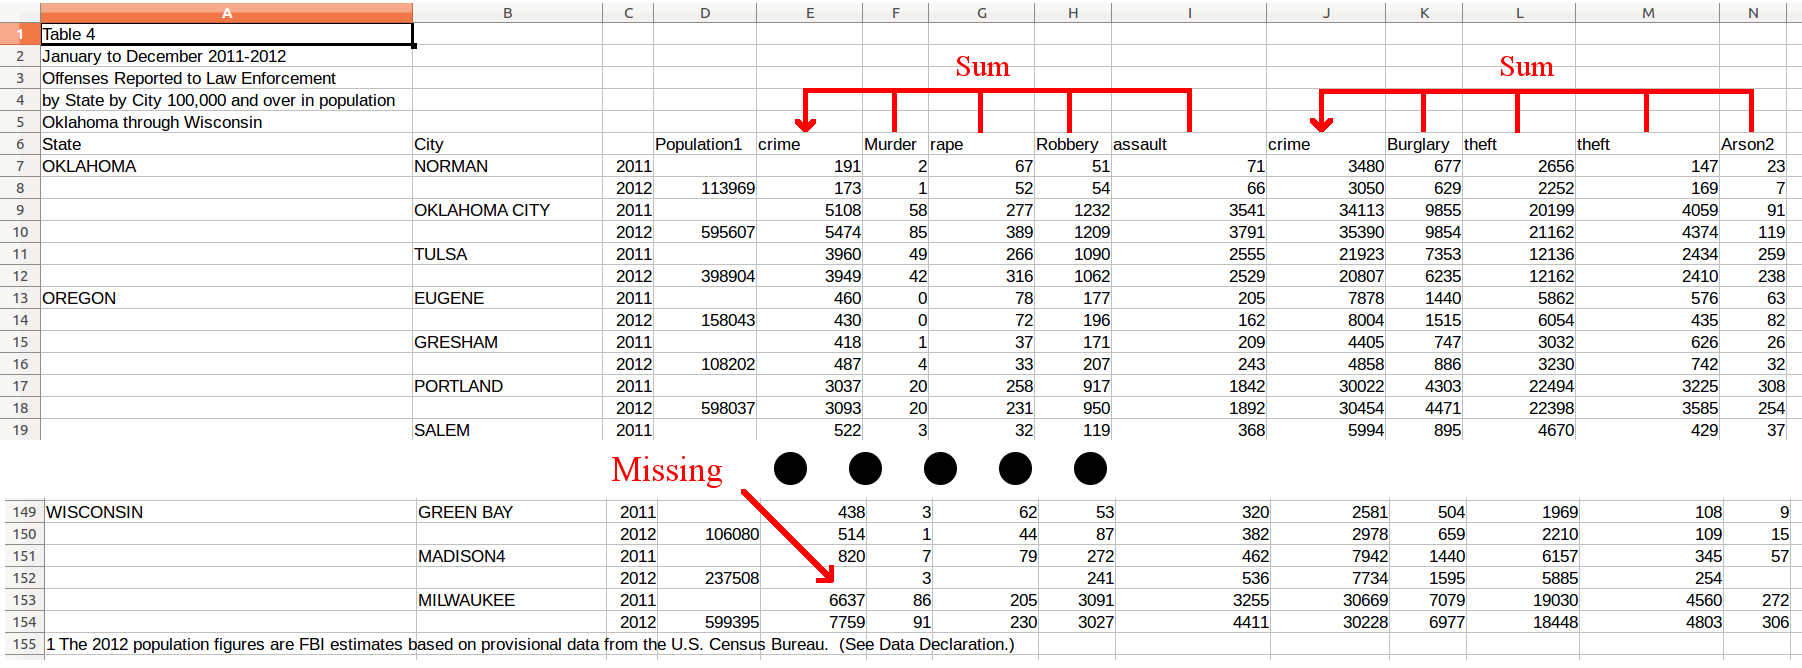
\includegraphics[width=0.85\textwidth]{figures/fbi_figure_highlighted.png}
  \end{center}
  \caption{Real world tabular constraint reconstruction: FBI crime statistics}
  \label{fig:fbi}
\end{figure*}

\subsection{Error detection}
We consider two cases of error detection.
The first setting is the \textit{online} detection of errors which is similar to the autocompletion setting.
However, instead of considering viable constraints, we look at \textit{conflict} constraints, i.e. constraints that were learned at time~$t_0$ but do not agree with the newly added data at time~$t_1$.
Such conflict constraints can indicate errors in the input.
Since conflict constraints could also be accidental constraints that are correctly invalidated by the new data, the size of the data at time ~$t_0$ should be large enough.

The second type of error detection is \textit{offline} and attempts to detect errors in a spreadsheet.
Consider, for example, a use case concerning crime statistics provided by the FBI.
An extract of the spreadsheet is depicted in Figure~\ref{fig:fbi}.
When run on this sheet, our system is able to detect the second sum constraint, however, a missing value prevents the first sum constraint from being learned.
A possible approach to detect such missing or wrong values is to look at a sample of the table that excludes the erroneous row and compare the constraints learned on this sample with the constraints learned by adding the row containing the mistake.
The sample needs to large enough such that we have enough confidence that the constraints are correct. For example, in Figure \ref{fig:fbi} all but one row satisfy the constraint, which is a strong indication that there is a constraint violation.
If we define the sample to be our data at time~$t_0$ and the added row to be the additional input at~$t_1$, this task can be formulated as online error detection and dealt with in the same way.
%Of course, generating large enough samples and rows (columns) to be added can be done in multiple ways.
%In the limited case of detecting single errors one can leave out every row (column), consider the remaining data to be the sample and
%and the left out row (column) to be new input.

\section{Related Work}\label{sec:related_work}
\sergey{key bullet points for Luc and possibly Samuel and me to make related work section}

\samuel{Two possible takes here: 1) recent interest in topics such as flashfill, etc -> sparked the idea for this project. This actually relates to constraint learning which has seen an uptick recently and is a subfield of long-established ILP. 2) ILP established field trying to learn structure / .., has been brought to the less traditional context (constraint learning), learning constraints / programs has been picked up by specific approaches such as flashfill etc which inspired this research}

\sergey{ECAI reference style file ignores their guideline and their guideline ignores what is written in the guidelines!}
flashfill, flashextract, flashmeta \cite{flashfill,flashextract,flashmeta}
\begin{itemize}
  \item their supervised vs our unsupervised approach
  \item they look for a single ``smallest'' solution, we enumerate them all
  \item they are looking for a function, we solve constraint satisfaction problems
  \item we do not assume classic row based data layout, we work in the tabular setting
\end{itemize}

sketch \cite{sketch}
\begin{itemize}
  \item look for a constant that would fill in the gap in a program
  \item tailored for programming languages
  \item similar to model checking
  \item looks for a single solution
  \item similar to constraint satisfaction and sat, where one is interested in a single assignment that works for any potential input
\end{itemize}

tabular \cite{tabular}
\begin{itemize}
  \item language based on the excel tables that specify probabilistic models
  \item a system for probabilistic inference and similarity mostly in the usage of excel
  \item probabilistic constraint satisfaction (?) and graphical models
  \item single solution again
\end{itemize}

modelseeker \cite{modelseeker} \sergey{Samuel, Luc, probably you would need elaborate here more in details}

\begin{itemize}
  \item not designed for excel-like data representation (type consistency, groups, etc)
  \item not designed for excel-like constraints (lookups, conditional ifs, etc)
  \item does not support user extensions (?)
\end{itemize}

claudien \cite{claudien} \sergey{Samuel, Luc, you would need to help with this one}

\section{Conclusions}\label{sec:conclusions}

% points: 1) can be a base for an actual plugin or a function in excel 2) novel problem and challenge for systems and constraint solvers 3) can be part of the complicated pipeline togehter with the header detection
Our goal is to automatically identify constraints in a spreadsheet.
We have presented and evaluated our approach, implemented as the system \sname, that is able to learn a large set of constraints from CSV data.
Moreover, the amount of redundant constraints found by the system is limited despite the lack of more sophisticated post-processing steps.

\paragraph{Future work}
There are multiple directions for future work on this topic.
Integrating the system in an interactive setting would offer users the possibility to easily receive and provide feedback.
Moreover, the system can be adapted to deal with additional types produce less redundant constraints through the use of (heuristic) filtering or post-processing.

Currently, the system only learns single constraints, however, extending our approach to nested constraints would allow more expressive concepts to be learned.
This shift would bring the approach in line with programming by example.

Aside from finding errors, the system can be extended to deal with noise and the ability to learn soft constraints.
Soft constraints are the (potentially weighted) constraints that hold only on some of the data.
This would extend the approach to new application domains as well as provide more native error detection.

\bibliographystyle{plain}
\bibliography{references}
\end{document}
%%%%%%%%%%%%%%%%%%%%%%%%%%%%%%%%%%%%%%%%%%%%%%%%%%%%%%%%%%%%%%%%%%%%%%
